\documentclass{ctexart}

\usepackage{graphicx}
\usepackage{geometry}
\geometry{a4paper, top=2.54cm, bottom=2.54cm, left=1.91cm, right=1.91cm}

\usepackage{tocloft} %模板中用了subfigure,不加此选项会产生冲突
\renewcommand{\cftsecleader}{\cftdotfill{\cftdotsep}}
\renewcommand{\contentsname}{\bfseries 目录}% 设置”目录“左对齐(xiao xing)

\usepackage[colorlinks, linkcolor = red]{hyperref}
\usepackage{enumitem}%  列表环境


\title{TTY 是什么?}
\author{ZiTai}
\date{\today}

\begin{document}
\maketitle

\clearpage
\tableofcontents

\clearpage
\section*{写在前面}
    在使用 Linux 时,偶尔会遇到 tty 这个术语。
    本篇文章旨在帮助你了解它是什么,它的意义是什么。

\clearpage
\section{术语 TTY 背后的历史}
    这一切都始于 19 世纪 30 年代的电传打印机。

    电传打印机可以让你通过电线发送/接收短信。
    它取代了莫尔斯电码(Morse code)通信,莫尔斯电码通信需要两名操作员才能进行有效的通信。

    电传打字机只需要一个操作员就可以轻松地传递信息。
    虽然它没有一个现代布局的键盘,但它的系统后来在 1901 年由唐纳德·默里(Donald Murray)改进,包括了一个类似打字机的键盘。

    默里密码(Murray code)减少了接线员发送信息的工作量。
    这使得电传打字机在 1908 年发展成为商用电传打字机成为可能。
    TTY 就是电传打字机(Teletypewriter)的缩写。

    电传打字机和普通打字机的区别在于,电传打字机是连接在通信设备上,用来发送打出来的信息。
    直到现在,电传打字机使人类在没有计算机的情况下通过电线进行更快的交流成为可能。

    以上,便是 TTY 的诞生。

\clearpage
\section{相对现代的概念}
    现在,你一定想知道,它是如何进入现代计算机和 Linux 的。

    首先,当电传打字机进入市场时,几年后半导体晶体管被开发出来,然后演变成微处理器,使计算机成为可能。
    最初的计算机没有键盘的概念。输入方法是打孔卡。

    \begin{figure}[htbp]
        \centering
        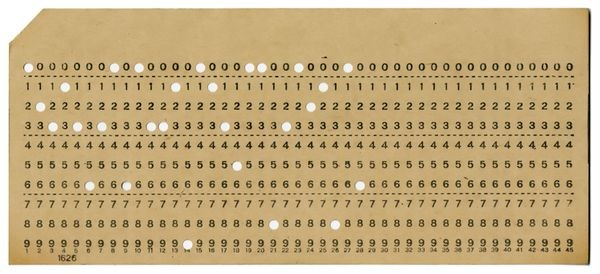
\includegraphics[width=0.80\textwidth]{images/punch-card-program.jpg}
        \caption{一种插入计算机而不是通过键盘输入的穿孔卡片计算机程序(TTY)}
    \end{figure}

    随着计算机的迅猛发展,批量输入卡最终被电传打字机取代,成为一种方便的输入/输出设备。

    \begin{figure}[htbp]
        \centering
        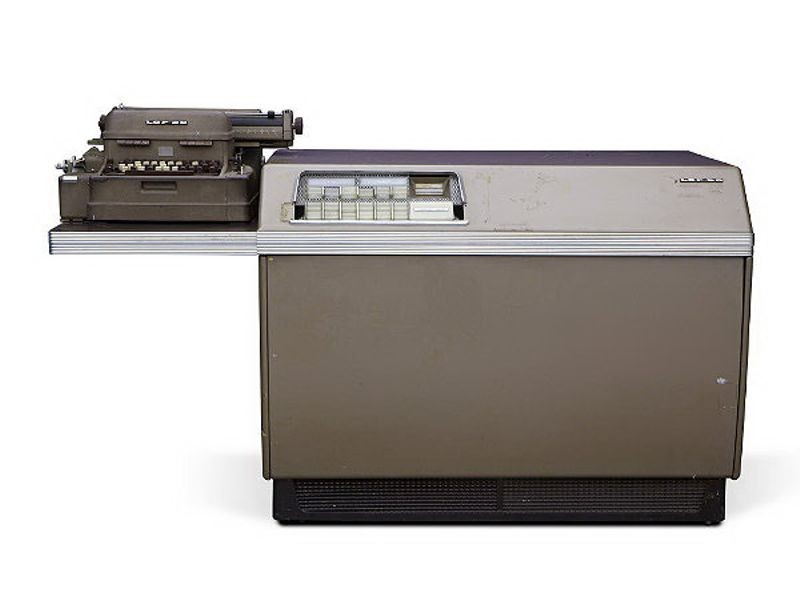
\includegraphics[width=0.50\textwidth]{images/LGP-30-early-computer-1956.jpg}
        \caption{1956 年的 LGP-30 计算机,附带了一个 TTY}
    \end{figure}

    随着技术的进步,电传打字机被电子技术虚拟化了。
    所以,你不需要物理的、机械的 TTY,而是虚拟的、电子的 TTY。

    早期的电脑甚至没有屏幕。
    东西被印在纸上,而不是显示在屏幕上(当时还不存在屏幕)。
    因此你看到的是“打印”这个词,而不是“显示”。
    随着技术的进步,图像后来被添加到终端中。
    换句话说,你可能听说过它们是视频终端(video terminals)。
    或者,你可以称它们为物理终端。
    然后,这些演变成软件仿真终端,具有增强的能力和特性。

    这就是所说的终端模拟器(terminal emulator)。
    例如,GNOME Terminal 或 Konsole(KDE’s terminal) 是您可以在 Linux 中找到的一些最好的终端模拟器。

\clearpage
\section{Linux 中的 TTY 是什么}
    在 Linux 中,TTY 是 Unix 和 Linux 中一个抽象的设备。
    有时它指的是物理输入设备,如串行端口,有时它指的是虚拟 TTY,允许用户与系统交互。

    TTY 是 Unix 和 Linux 中的一个子系统,它通过 TTY 驱动程序在内核级别实现进程管理、行编辑和会话管理。
    在编程方面,你可能需要深入研究。
    但是,考虑到本文的范围,这可能是一个容易理解的定义。

    如果你很好奇,你可以看看这个这份资料:
    \href{https://www.linusakesson.net/programming/tty/index.php?ref=itsfoss.com}{TTY Demystified},
    它试图澄清你想知道的关于 Unix 和 Linux 系统中 TTY 的所有技术细节。

    实际上,无论何时启动终端仿真器或在系统中使用任何类型的 shell,
    它都会与称为伪TTY 或 PTY(pseudo-TTY) 的虚拟 TTY 进行交互。
    你只需在终端模拟器中输入 TTY 即可找到相关的 PTY。

\clearpage
\section{如何在Linux下访问TTY}
    在 Linux 中访问 TTY 很容易。
    在大多数发行版中,你可以使用以下键盘快捷键获得 TTY 屏幕:

    \begin{itemize}[itemindent=1em]
      \item CTRL + ALT + F1 – Lockscreen
      \item CTRL + ALT + F2 – Desktop Environment
      \item CTRL + ALT + F3 – TTY3
      \item CTRL + ALT + F4 – TTY4
      \item CTRL + ALT + F5 – TT5
      \item CTRL + ALT + F6 – TTY6
    \end{itemize}

    你最多可以访问 6 个 tty。其中,前两个快捷方式指向发行版的锁定屏幕和桌面环境。

\clearpage
\section{什么时候在 Linux 中使用 TTY}
    在图形化桌面环境死机的情况下,从 TTY 重新安装桌面环境有助于解决该问题。

    或者,你也可以选择在 TTY 中执行任务,
    例如更新 Linux 系统和类似的任务,在这些任务中,你不希望图形问题中断你的进程。

    最坏的情况是,如果图形用户界面没有响应,你可以转到 TTY 并重新启动计算机。

    有些用户还喜欢在 TTY 的帮助下执行大文件传输。

\clearpage
\section{将 TTY 作为 Linux 中的命令使用}
    你在终端模拟器(terminal emulator)中输入 TTY 时,
    如手册(man)里所描述的那样,它将打印连接到标准输入的终端的文件名。
    换句话说,要知道你所连接的 TTY 数字,只需键入 TTY 命令。
    而且,如果有多个用户远程连接到 Linux 机器,你可以使用 who 命令检查连接到的其他用户。

\end{document}